Our model identifies two types of organisms belonging to the coral reef ecosystem as the most relevant organisms relating to the long term stability of a coral reef: macroalgae and algal turf. The interactions between these organisms can be described in the following directed graph, where the direction denotes which organism is benefited by the interaction,

%\begin{wrapfigure}{L}{2.82in}\end{wrapfigure}

\hspace{1.5em} 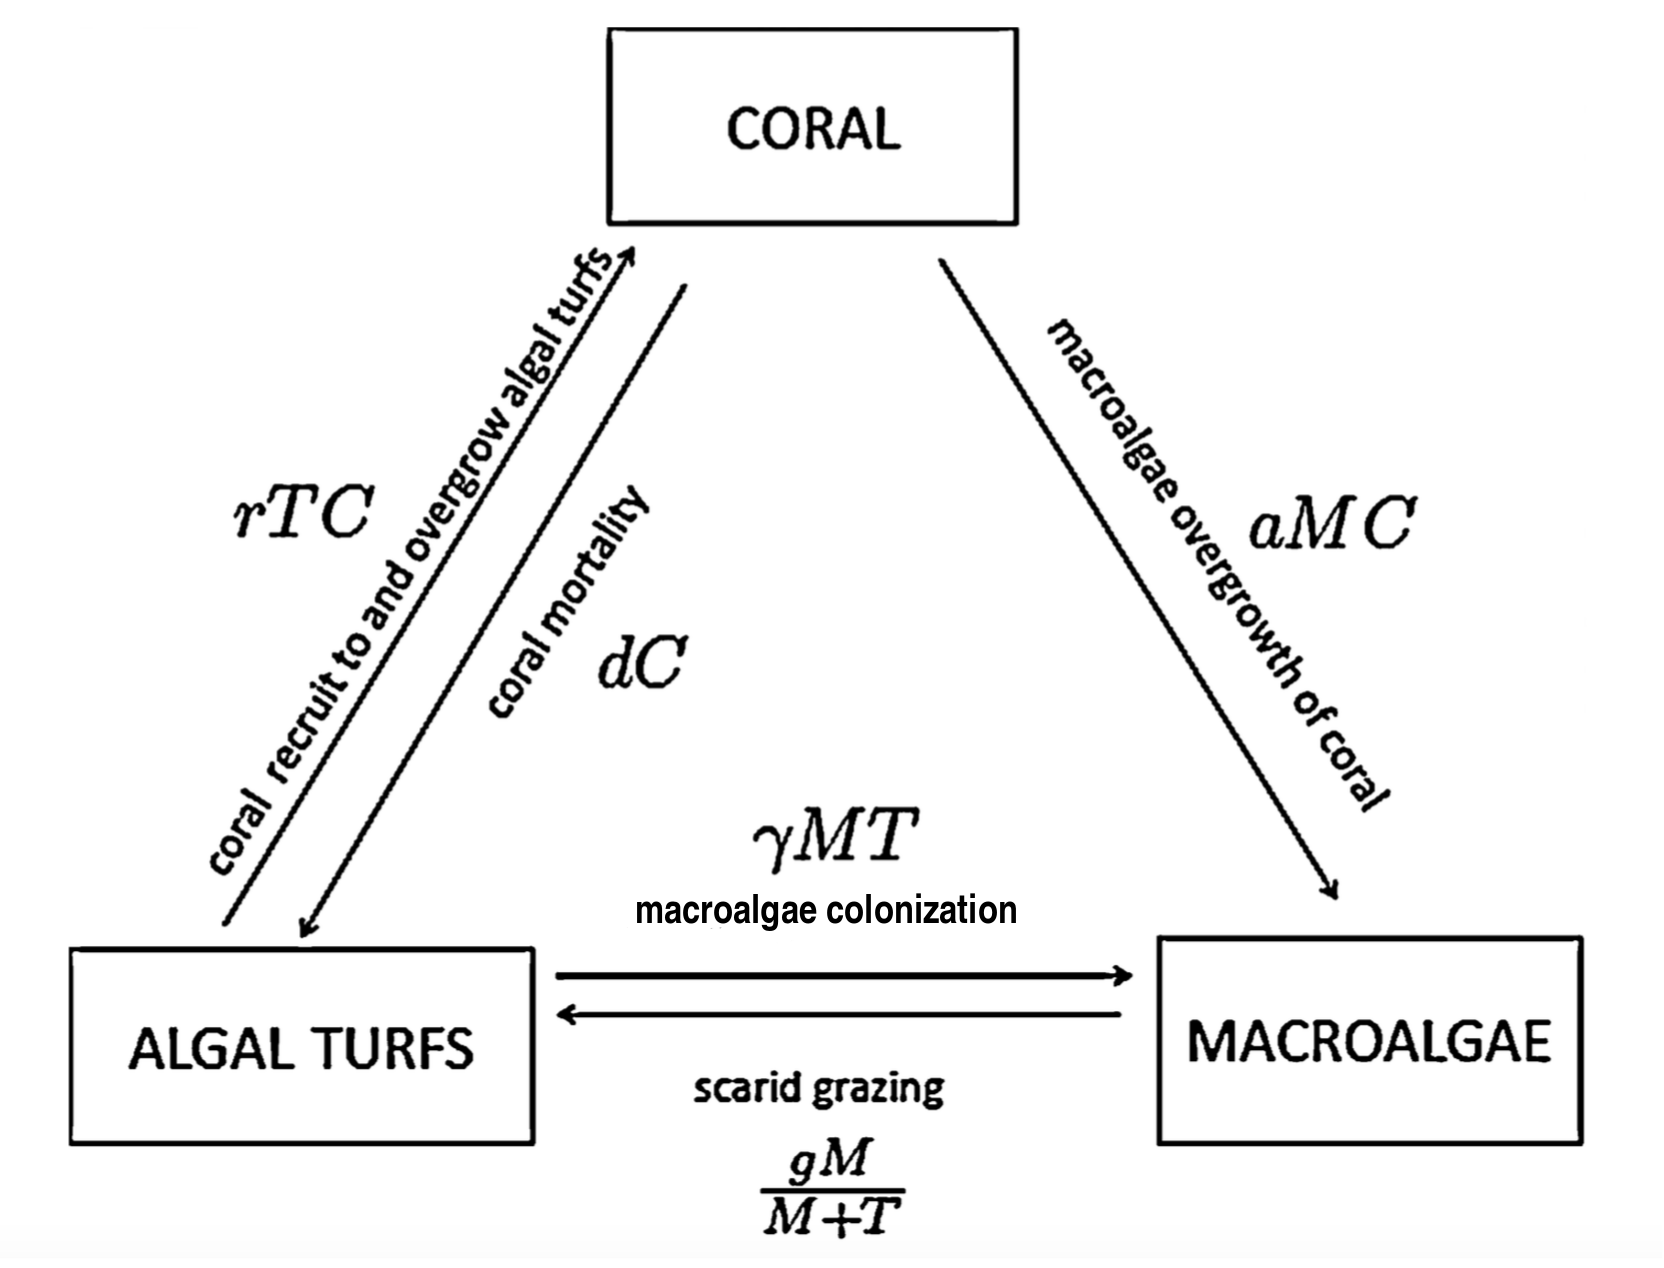
\includegraphics[scale=.125]{coral-reef-triangle.png}\\

We began by studying the following delay differential equation (DDE) model:
$$\begin{cases}
  \begin{array}{rl}
    \frac{dM}{dt}\hspace{-.8em}&=aMC - \frac{gM(t-\tau)}{1-C(t-\tau)} + \gamma M (1-M-C),\\
    \frac{dC}{dt}\hspace{-.8em}&=rC(1-M-C) - dC - aMC,
  \end{array}
\end{cases}$$ where  $\tau\geq0$ is a fixed time delay observed in the growth of algal turf upon the grazing of macroalgae; 
$r$ is the rate corals overgrow upon algal turfs; 
$d$ is the mortality rate of corals; 
$a$ is the rate that macroalgae overgrow upon corals; 
$\gamma$ is the rate that macroalgae spread over algal turfs, and; 
$g$ is the indiscriminate grazing rate of scarid,
and we also assume $a<d<\gamma<r<2\gamma$ and $0<g<\gamma$ \cite{Hastings}. 

Notice that algal turf is given by $1-C-M$, as we assume that $M+C+T=1$, given that $\frac{dM}{dt}+\frac{dC}{dt}+\frac{dT}{dt}=0$. By analyzing the nullcline of this system, three equilibrium points are discovered:\begin{inparaenum}[(A)]
\setcounter{enumi}{13}
\item $(0,0)$;\setcounter{enumi}{1}
\item $(0,1-\frac{g}{\gamma})$, and;\setcounter{enumi}{3}
\item $(1-\frac{d}{r},0)$,
\end{inparaenum} and in Li et. al, 2014, these equilibrium points were discovered to be unstable, stable, and stable, respectively.

We extended the DDE model to a Stochastic DDE Model (SDDE) by accounting for noise in scarid grazing of macroalgae by adding a noise term in the derivative of $M$, 
$$\begin{cases}
\begin{array}{rl}
dM\hspace{-.8em}&=(aMC - \frac{gM(t-\tau)}{1-C(t-\tau)+\gamma M T})dt+{\color{red}\beta M(1-M)dW},\\
dC\hspace{-.8em}&=(rTC  - dC - aMC)dt,\\
\end{array}
\end{cases}$$ where $\beta$ is constant. The coefficient $M(1-M)$ is used so that noise has the greatest impact when $M$ is the midpoint of the interval $[0,1]$.

We denote the initial condition with $\theta$ in radians, such that $C=\sin(\theta)$ and $M=\cos(\theta)$. The impact of noise on the stability of the equilibrium points was studied using Monte Carlo simulations with varying values for $g\in[0.2,0.8]$, $\tau\in[0.5,1]$, $\beta\in[0,1]$, and $\theta\in(0,\frac{\pi}{2}]$.